\subsection{Komponentbeskrivelse}\label{sec:blockdescription}
Her beskrives komponenterne som blev vist på blokdiagrammet på side~\pageref{fig:blockdiagram}. 

\subsubsection{Bruger}
Brugeren af systemet vil være interesseret i at kunne indhente forskellige målinger fra et system, som kan være placeret på en vilkårlig position, så længe der er mobildækning.

\subsubsection{MC35}
Siemens MC35 GSM/GPRS Modem (vist på figur~\ref{fig:devicegsm}) er i projektet anvendt til at sende og modtage sms beskeder, som gør kommunikation mellem bruger og system mulig. Under udvikling har to forskellige enheder været brugt. Med den første enhed var der en del inkonsistens i opførsel under udvikling, men da denne enheds blev udskiftet stoppede problemerne og debugging af problemer blev meget lettere.

\begin{figure}[h]
	\centering
	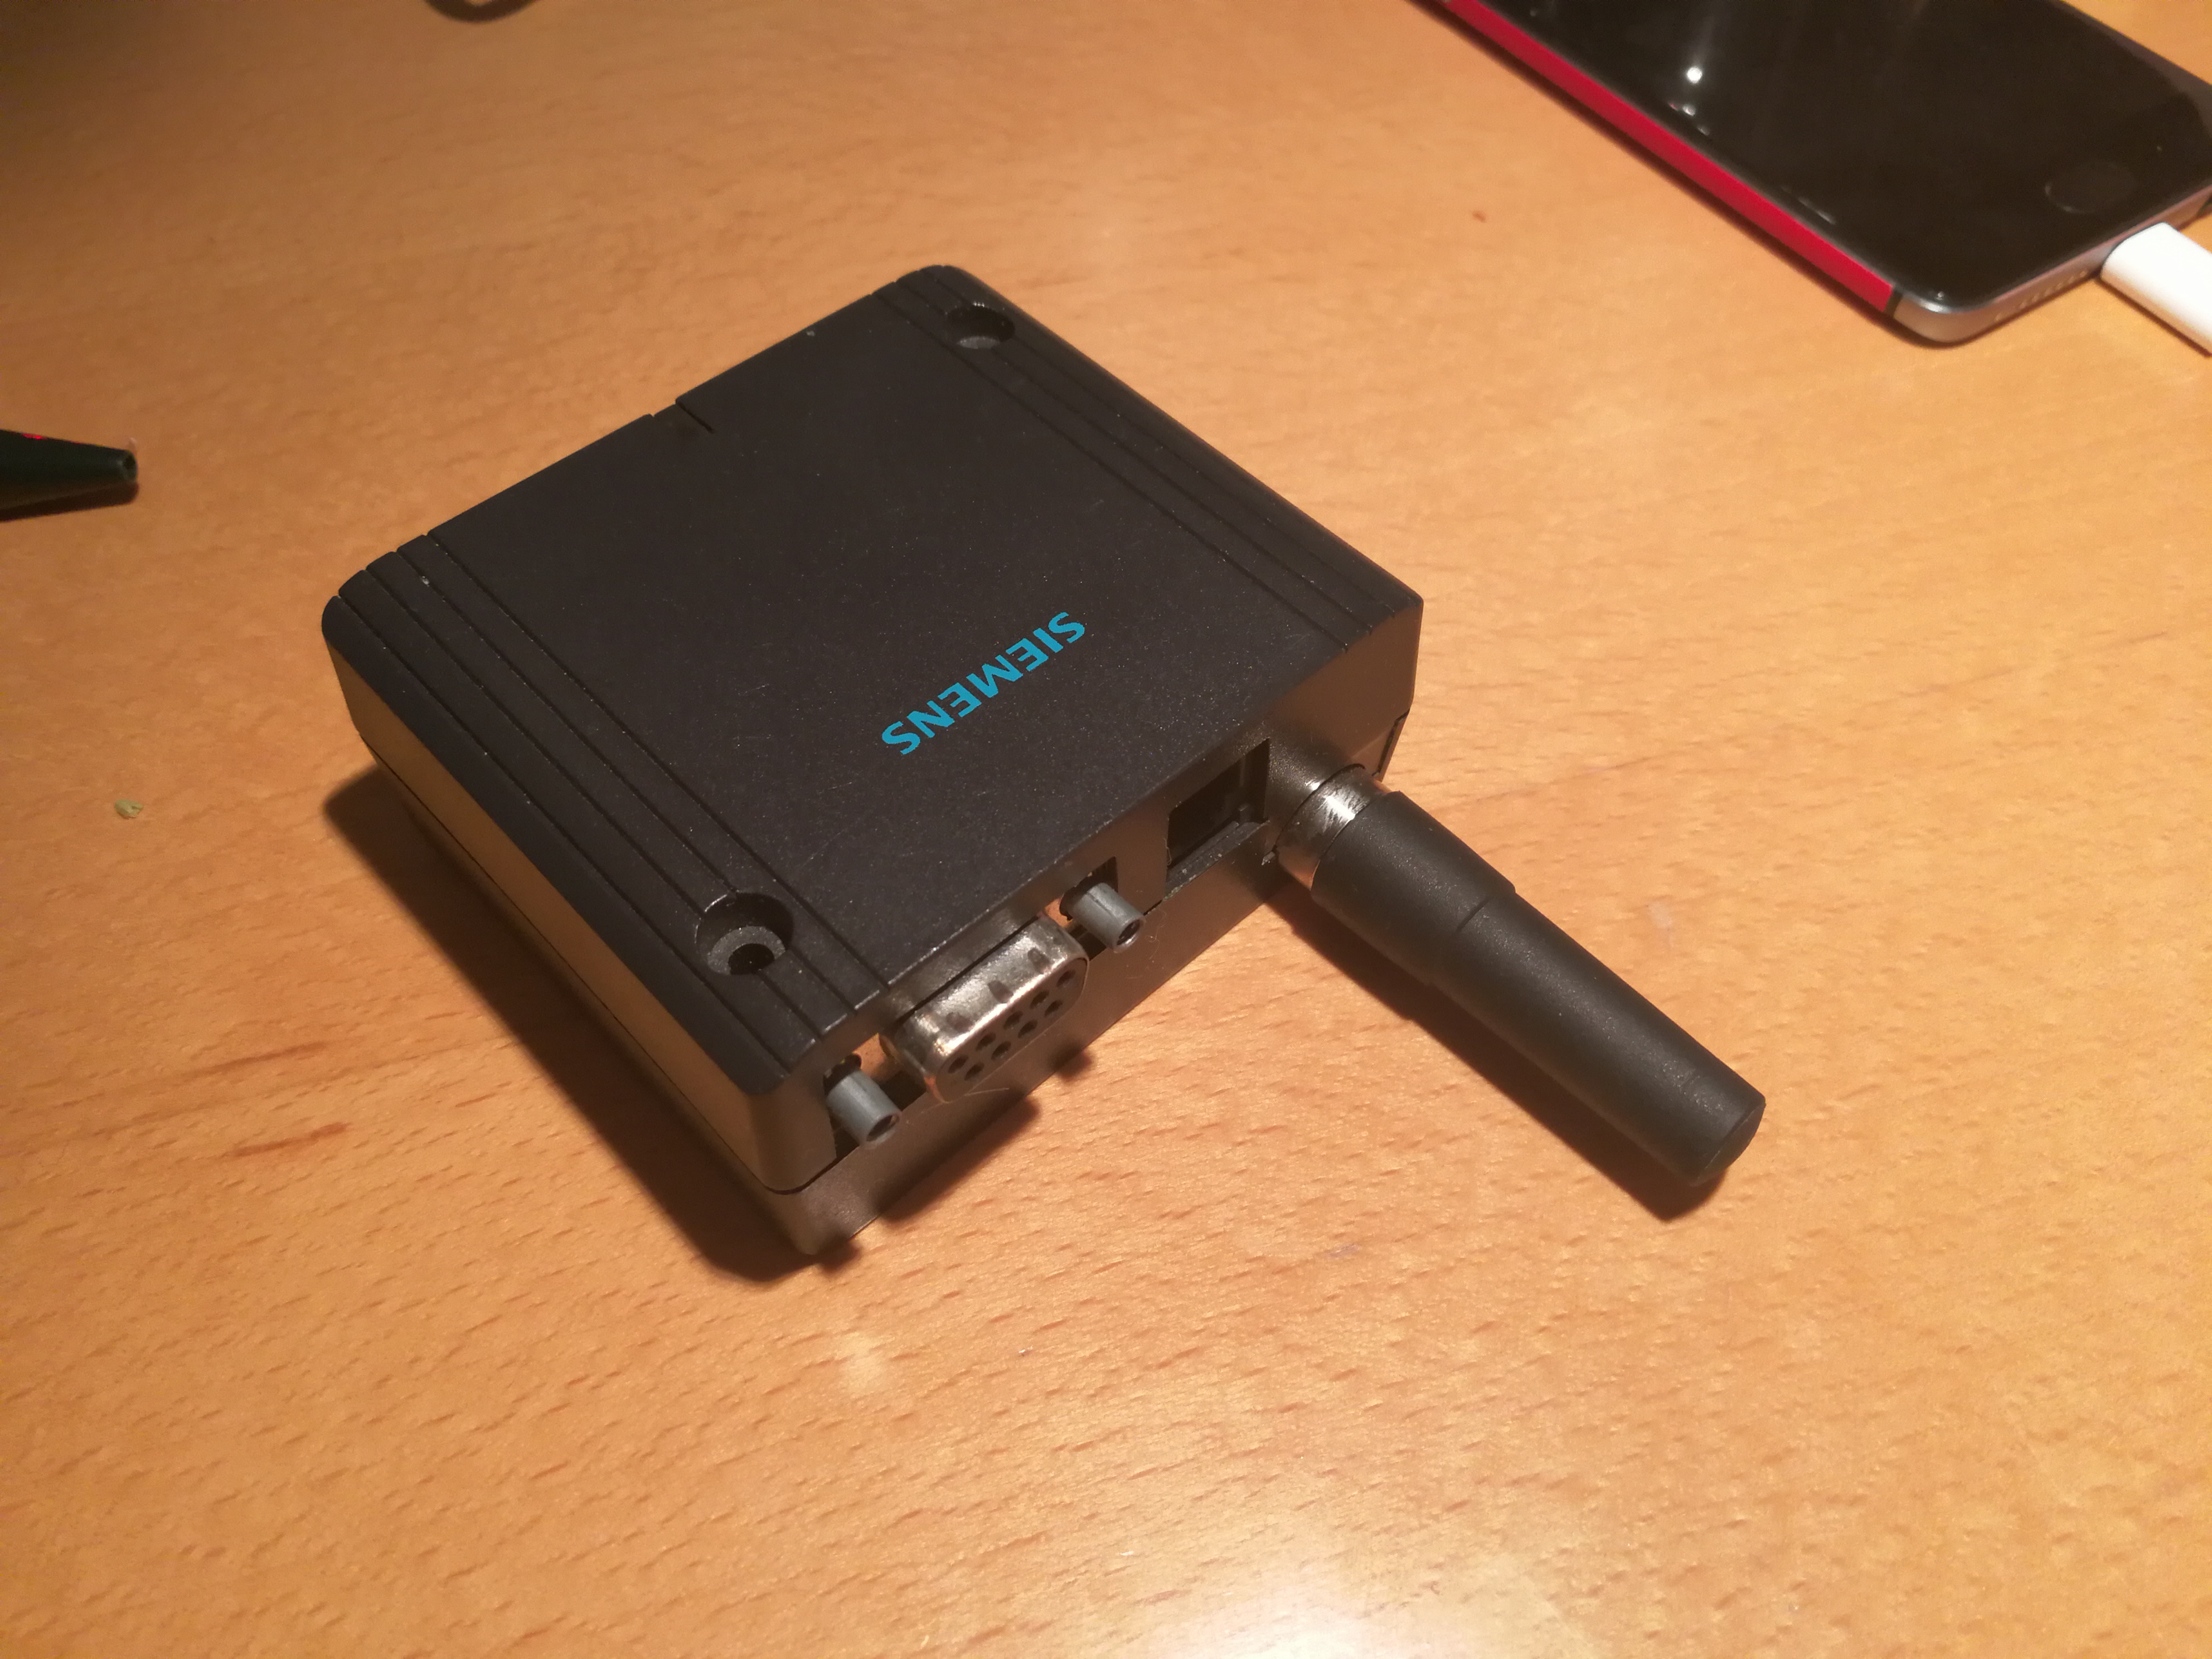
\includegraphics[width=0.7\linewidth]{figs/device_gsm.jpg}
	\caption{Siemens MC35 GSM/GPRS modem.}
	\label{fig:devicegsm}
\end{figure}

\subsubsection{ATmega32}
ATmega32 er brugt i forbindelse med STK500 boardet, som hovedkomponent i udviklingen. Denne er vist på figur~\ref{fig:deviceatmege32}. Boardet interfacer med GSM modemet via UART og fortolker de modtagne kommandoer før der kan anmodes om de ønskede målinger fra BMP modulet.

\begin{figure}[h]
	\centering
	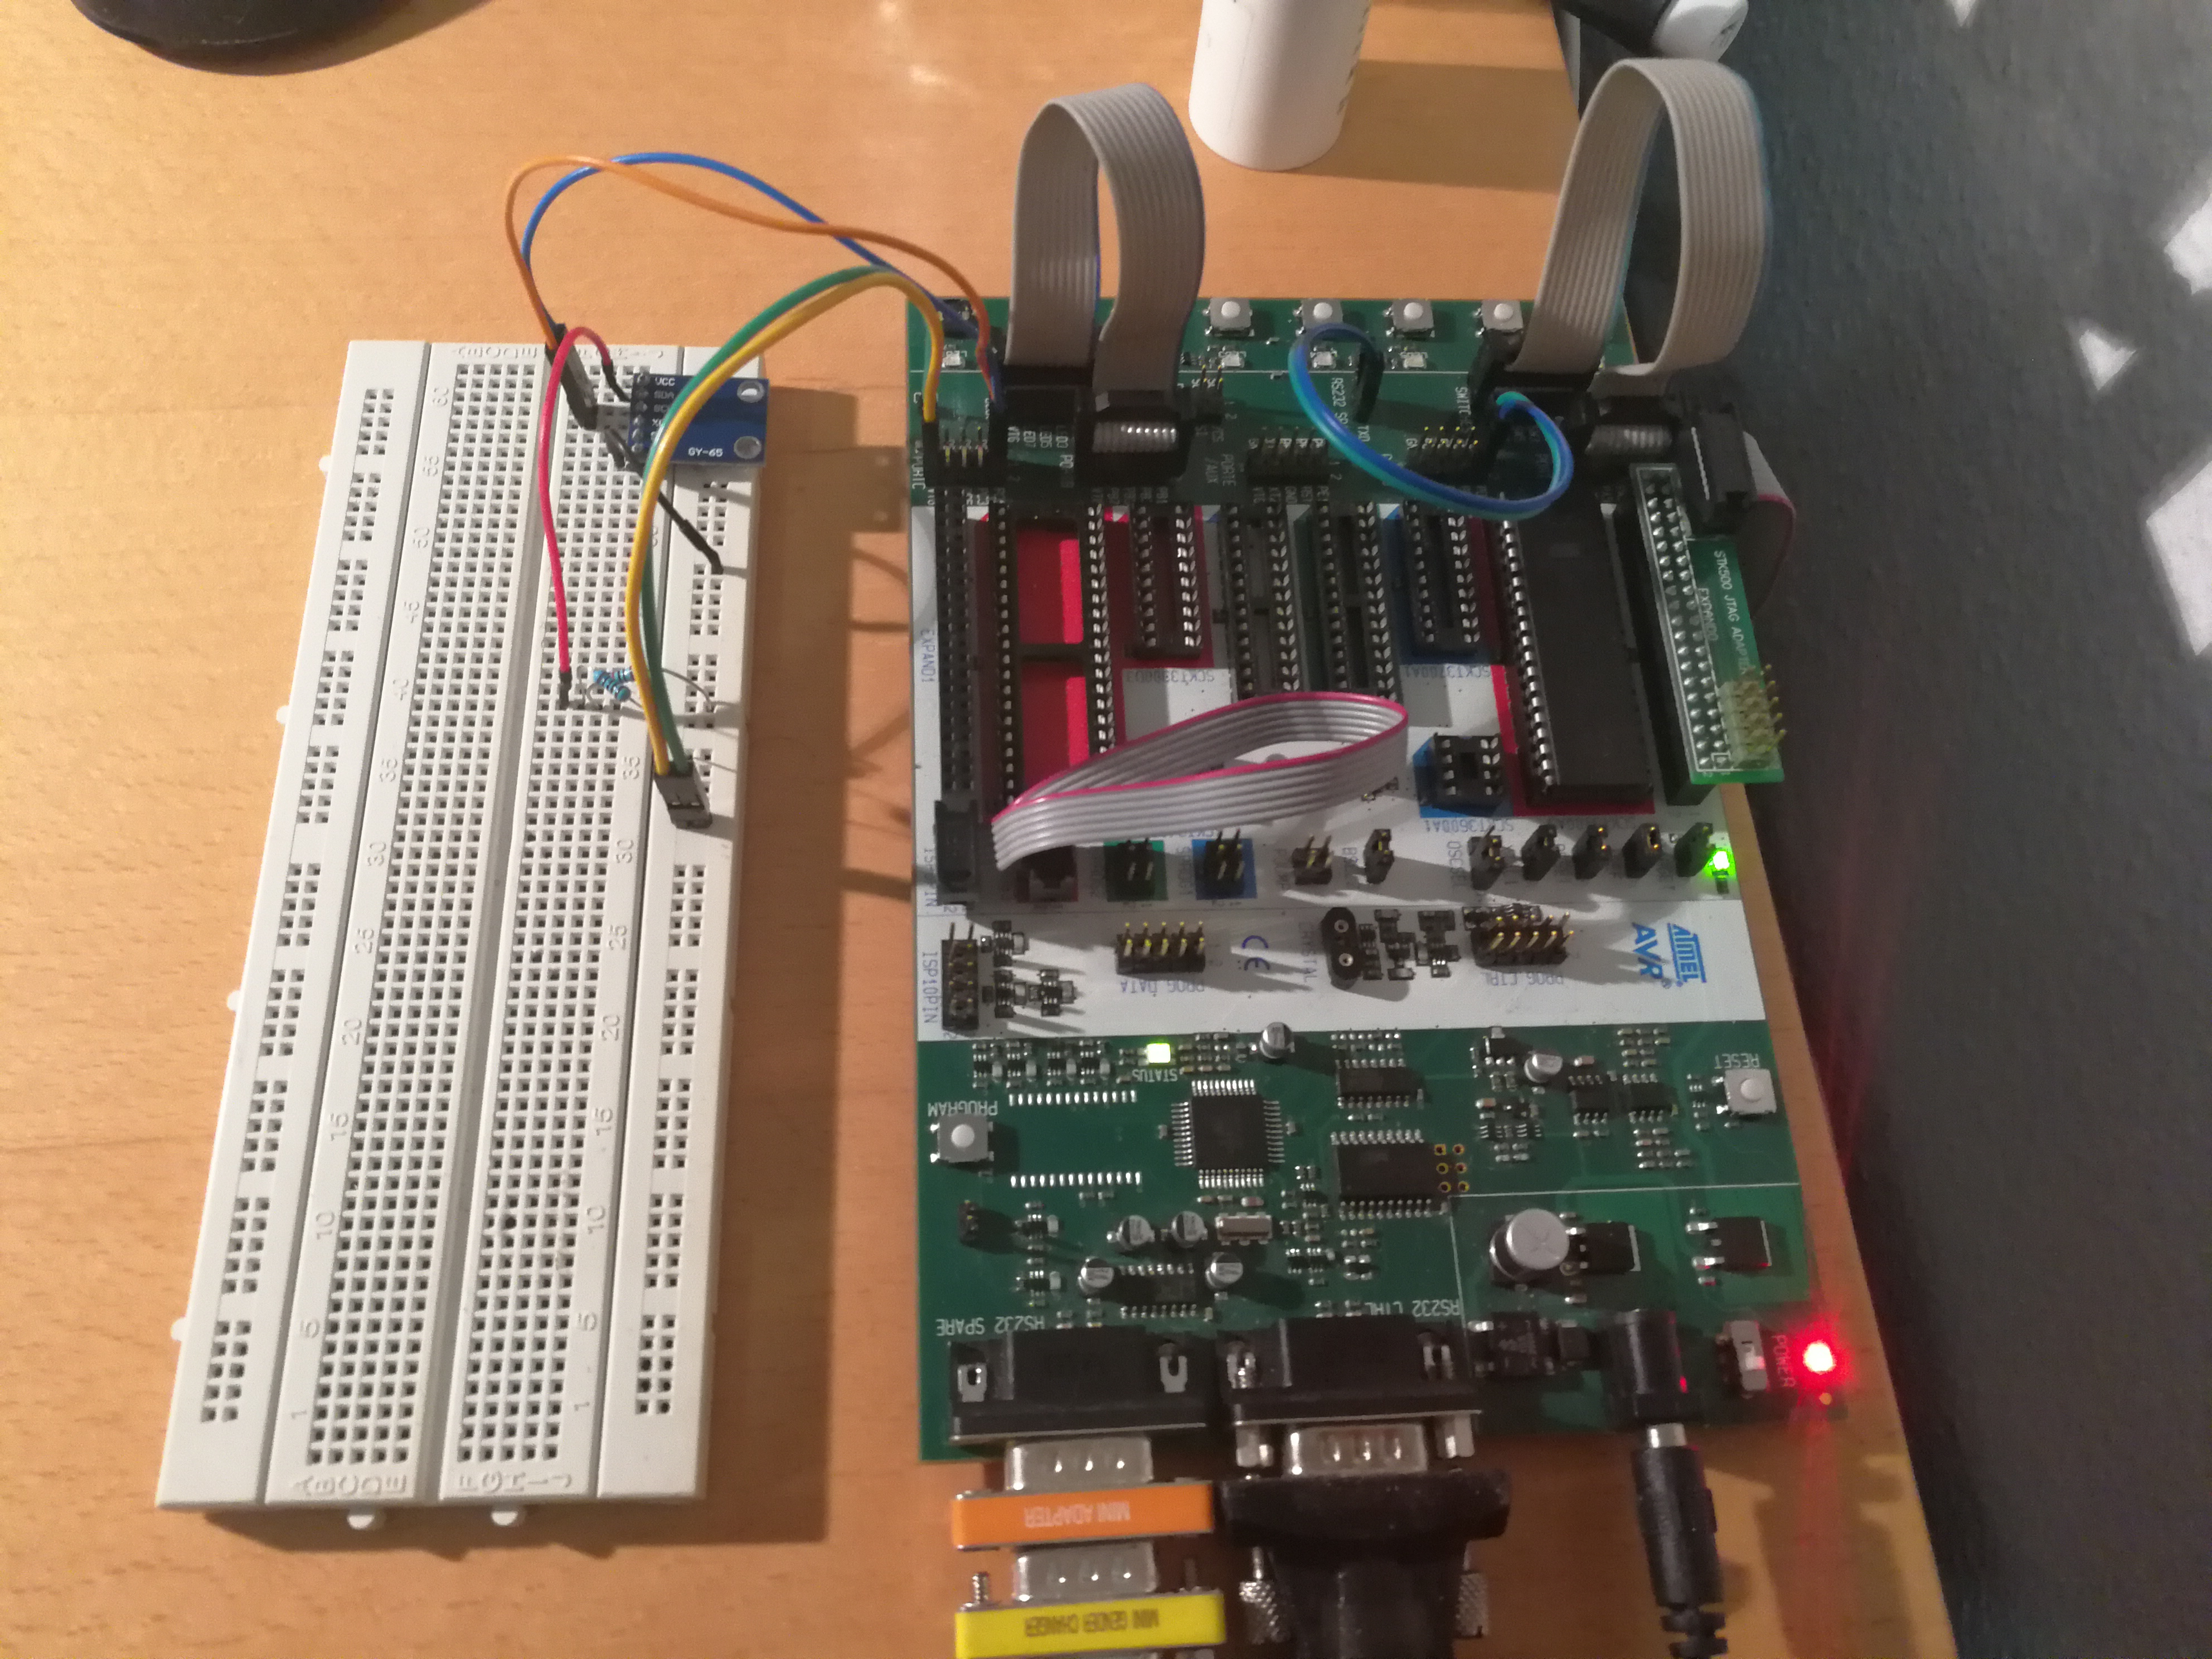
\includegraphics[width=0.7\linewidth]{figs/device_atmega32.jpg}
	\caption{STK500 board opsætning med ATmega32.}
	\label{fig:deviceatmege32}
\end{figure}

\subsubsection{BMP}
BMP08 modulet er brugt til at foretage målingerne og kommunikerer med ATmega32 over I2C. Den er i stand til at måle temperatur, lufttryk og altitude. Disse tre forskellige målinger kan så anmodes af ATmega32 og senders ud til brugeren. Vist på figur~\ref{fig:devicebmp}.

\begin{figure}[h]
	\centering
	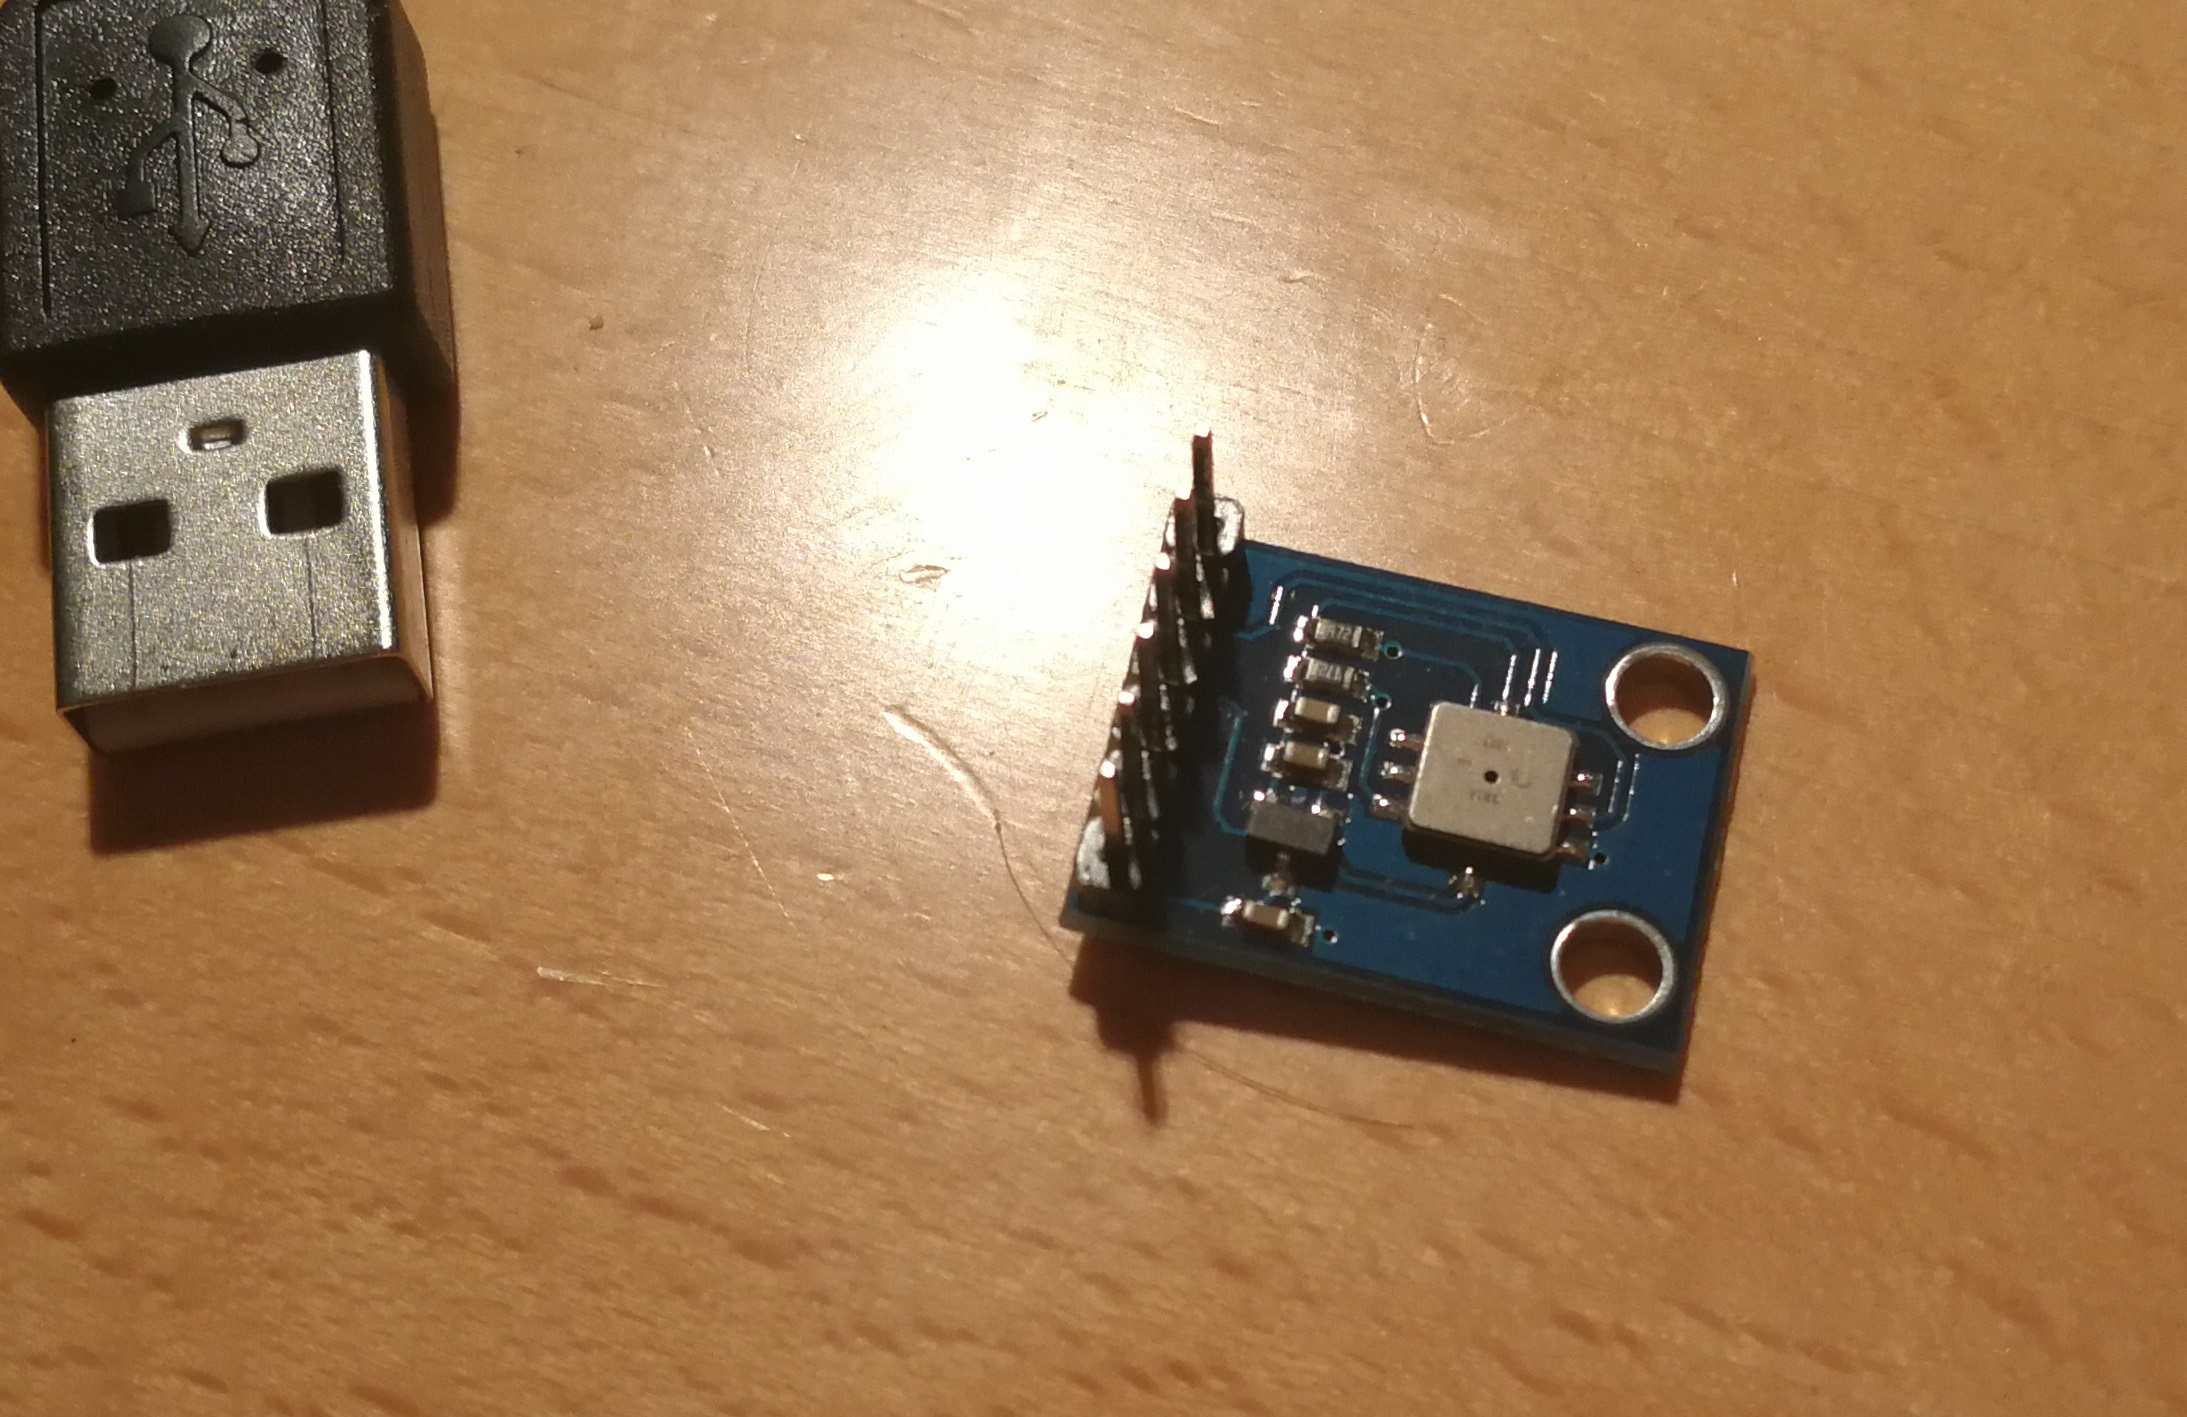
\includegraphics[width=0.7\linewidth]{figs/device_bmp.jpg}
	\caption{BMP085 digital trykføler.}
	\label{fig:devicebmp}
\end{figure}
